\chapter{Descrierea aplicatiei AudIT}
Adaptarea la noile paradigme tehnologice ne impune tuturor o provocare,mai mult sau mai putin difica, institutiile publice statului confruntandu-se zilnic cu aceasta problema, este nevoie cat mai repede de o solutie eficienta care va rezolva aceasta problema.
\par Prima sectiune a acestei lucrari urmareste sa exploreze in detaliu cum platforma AudIT se aliniaza si contribuie la actiunea de transformare si adaptare digitala in sectorul public, analizand componentele cheie ale aplicatiei in raport cu problemele pe care aceastea incearca sa le rezolve.


\section{Problema adresata}
Digitalizarea, potrivit definitiei este procesul de transformare a informatiilor dintr-un format analogic, hartii, intr-un format digital,biti. De fapt, acest procedeu constituie o adevarata noua paradigma in materie de algoritmi administrativi, sensul de derulare al intregului sistem si metodele utilizate de catre factorul uman in dezvoltarea solutiilor.
\par In decursul discutiilor  cu tatal meu, auditor public, am descoperit impreumna numeroase 
puncte nevralgice in metodele si solutiile folosite de auditorii publici din Romania pentru a duce la capat anumite intrebuintari de serviciu. Acestea pot parea nesemnificative pe moment, dar observand fenomenul la scara larga, de exemplu pe intreg parcurul unei misiuni de audit public, care poate dura pana la 6 luni, constatam faptul ca intreg procesul si eficienta auditorului sunt major incetinite de aceste imperfectiuni.
\par Una dintre cele mai mari probleme prezente in procesul de audit public, si cel mai probabil in majoritatea institutiilor publice din tara, este nevoia de a folosi si a administra inventarul a multor documente oficiale, pierzand astfel mult timp in identificarea documentului corespunzator actiunii sau activitatii pe care auditorul vrea o sa efectueaze, ulterior pierzand si mai mult timp in completarea si in comunicarea si transmiterea acestui act catre reprezentantul agentiei sau departamentul auditat.De acest lucru este strans legata si problema comunicarii intre partile care participa la misiunea de audit public,aceasta realizandu-se in majoritatea cazurilor prin intermediul postei iar uneori daca distanta permite chiar prin intermediul unor 'curieri umani'. 
\par  Avand in vedere aceste vulnerabilitati din sistemul public de audit, platforma web AudIT a fost conceputa pentru a raspunde nevoii de adaptare si transformare digitala, incercand in acelasi timp sa imbunatateasca protocoalele si procesele interne, astfel permitand factorului uman sa isi indeplineasca sarcinile intr-un mod mult mai usor si rapid.

\section{Solutia propusa}
Platforma Web AudIT este conceputa ca o solutie inovatoare asupra provocarilor datorate digitalizarii in instituiile publice, oferind un set de instrumente si functionalitati care fac mult mai accesibila si fluenta munca auditorului public cat si cea a reprezentantilor institutiilor audidate.
\par Aplicatia are ca si scop principal cresterea eficientei in procesul de audit public, prin implementarea diferitelor functionalitati care vor imbunatati drastic accesul utilizatorilor la informatii si documente relevante, vor creste nivelul eficientei, auditorii concentrandu-se pe aspecte esentiale ale auditului, fara a-si consuma  astfel timpul si energia pe numeroase sarcini care se pot dovedi repetitive, amanuntite si obositoare in final	respectiv va facilita un mod de comunicare eficace intre persoanele care iau parte la misiunea de audit.



\section{Functionalitatile aplicatiei}
Subsectiunile care vor urma o sa prezinte in detaliu functionalitatile de baza ale platformei,
modul in care acestea au fost implemnentate, cat si dificultati si provocari ulterioare in ceea ce priveste facilitatile oferite de acestea.

\subsection{Autentificarea pe platforma}
Prima interactiune a fiecarui utilizator cu platforma web o constituie pagina de autentificare, care asigura faptul ca accesul la functionalitatile aplicatiei este restrictionat doar celor care detin sau doresc sa isi creeze un cont pe aceasta aplicatie.\\
Procesul de creare a unui cont nou este conceput astfel incat sa se ajusteze pe necesitatile de securitate de baza ale institutiilor publice.
\par  Presupunand faptul ca fiecare angajat al unui departamant dintr-o institutie a statului detine o adresa de email cu domeniul institutiei de care apartine, tot ce treuie sa faca noul potential utilizator este sa se foloseasca de aceasta adresa de email ca sa isi creeze un cont nou. Contul nou este creat cu drepturi limitate, acesta neavand acces la nici o resursa care apartine de institutia sa pana in momentul cand un reprezentant al institutiei nu ii valideaza contul.
 
 	\vspace{0.5 cm}
 \begin{figure}[h]
 	\centering
 	
 	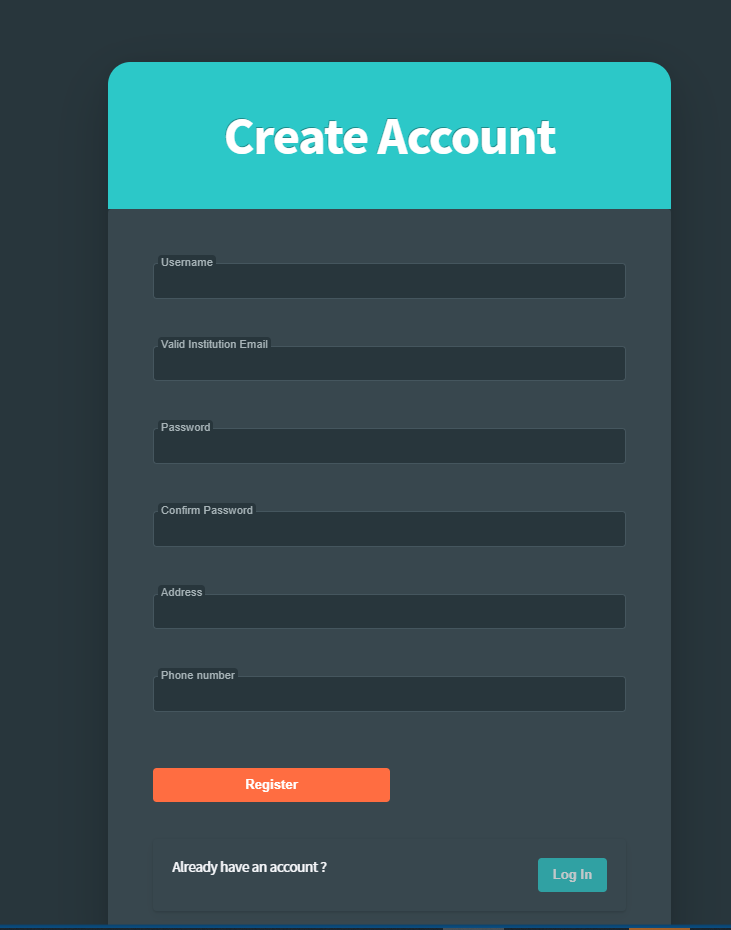
\includegraphics[width=0.5\textwidth]{c1/register.png}
 	\caption{Inregistrarea  pe platforma}
 \end{figure}
 
Aceasta metoda de autentificare se bazeaza pe o  configurare initiala a unor utilizatori cu drepturi elevate, reprezentantii departamentelor, carora li se ofera capacitatea de a verifica noii utilizatori care se inregistreaza pe platforma utiliand domeniul departamentului in cauza.Fiind pe o parte un mod in plus prin care se limiteaza accesul utilizatorilor la anumite resurse pana cand identitatea acestora este confirmata, este pe de alta parte un pas necesar care nu prezinta momentan un sistem de automatizare a verificarii identitatii utilizatorilor, eliminand astfel nevoia unei configurari initiale a platformei.
	\vspace{0.5 cm}
\begin{figure}[h]
	\centering
	
	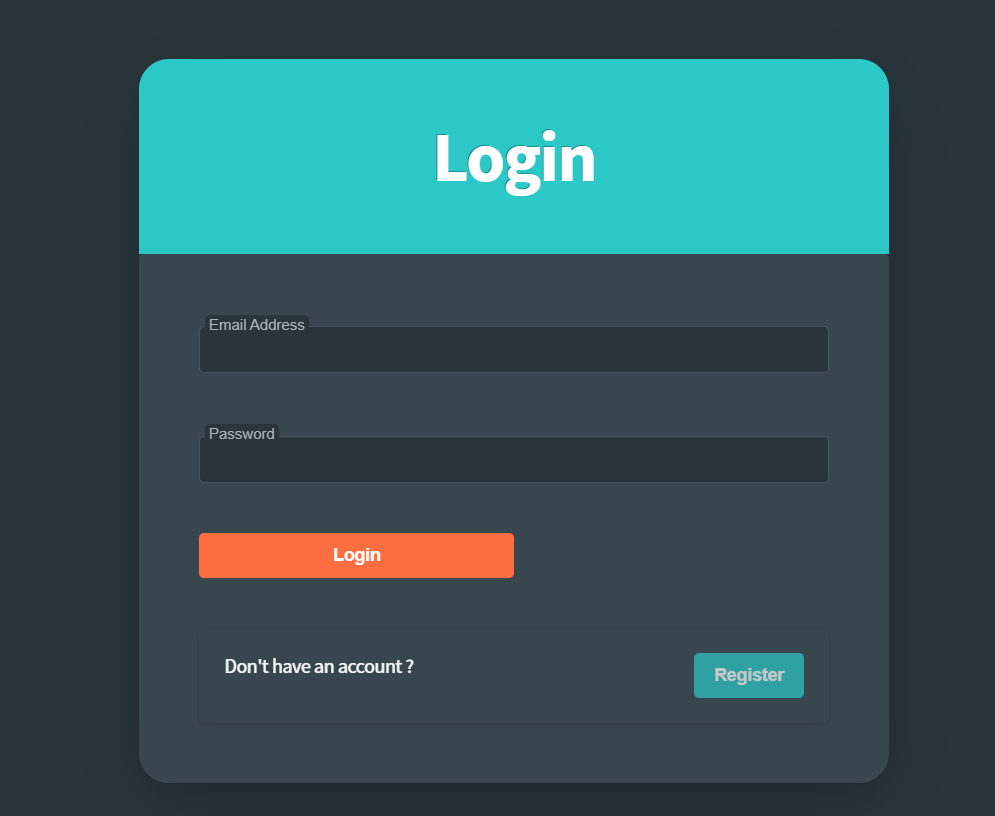
\includegraphics[width=0.5\textwidth]{c1/login.png}
	\caption{Autentificarea pe platforma}
\end{figure}

\subsection{Verificarea actiunilor utilizatorilor}
In cadrul aplicatiei, accesul la fiecare entitate este protejata prin implementarea unor liste de acces care definesc permisiunile de scriere si de citire asupra respectivei entitati.Acest lucru se asigura ca initial, fiecare utilizator are drept de scriere si de citire doar asupra resurselor create de acesta pe platforma, ulterior acesta avand posibilitatea de a acorda sau a primi acces de scriere sau citire asupra altor resurse aflate pe platforma.
	
De asemenea, este implementat si un sistem de roluri care restrictioneaza si acestea la randul lor accesul la diferite functionalitati ale aplicatiei, astfel spre exemplu, un utilizator cu rol de reprezentant al unei institutii nu va putea accesa paginile referitoare la crearea sau editarea unei misini de audit.
In plus, pentru o conformitate si pentru o evidenta sporita asupra actiunilor utilizatorilor asupra resurselor de pe platforma este implementat un sistem de auditare al entitatilor, toate operatiile de creare, modificare si stergere fiind salvate.

\subsection{Pagina de start}
Pagina de start este locul implicit unde un utilizator este redirectionat atunci cand autentificarea sa pe aplicatie este cu succes. Aceasta ii prezinta auditorului ultimele modificari la resursele la care are acces, o lista de notificari pe care acesta le-a primit din partea reprezentantilor institutiilor la care auditorul are misiuni de audit in desfasurare cat si diferite butoane de navigare catre pagini cheie din aplicatie, astfel oferind o interactiune mai usoara cu platforma AudIT.

\subsection{Gestionarea misinilor de audit public}
In cadrul procesului de audit public, o gestioneare eficienta a misiunilor, atat curente cat si din trecut, este esentiala pentru o experienta cat mai naturala si intuitiva a utilizatorului pe platforma.

Crearea unei noi misiuni de audit este similara cu crearea unui nou proiect, auditorul specificand numele noii misiuni de audit, institutia respectiv departamenul asupra caruia se realizeaza noua misiune de audit.

	\vspace{0.5 cm}
\begin{figure}[h]
	\centering
	\begin{minipage}{.5\textwidth}
		\centering
		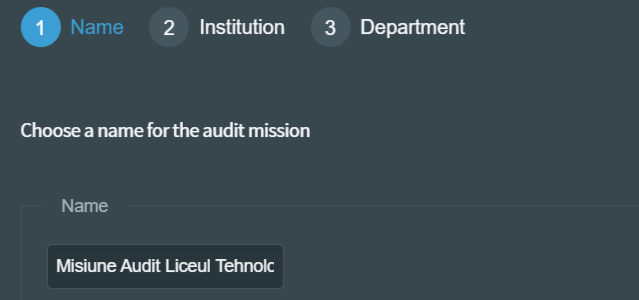
\includegraphics[width=.9\linewidth]{c1/pas1_creare_misiune.png}
		\caption{Stabilirea numelui}
		
	\end{minipage}%
	\begin{minipage}{.5\textwidth}
		\centering
		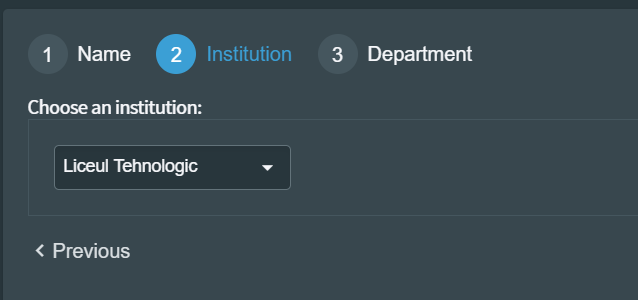
\includegraphics[width=.9\linewidth]{c1/pas2_creare_misiune.png}
		\caption{Selectarea institutiei}
	
	\end{minipage}
	\vspace{0.5 cm}

	\centering
	
	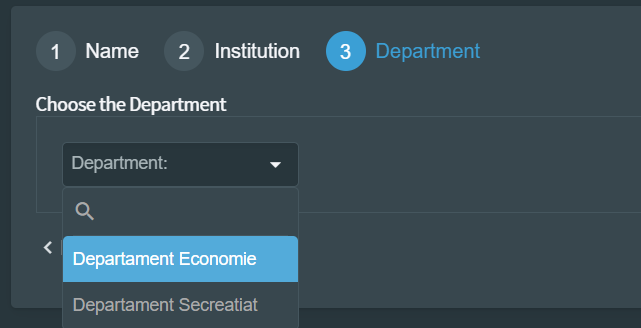
\includegraphics[width=0.5\textwidth]{c1/pas3_creare_misiune.png}
		\vspace{0.5 cm}
	\caption{Selectarea departamentului}
	
	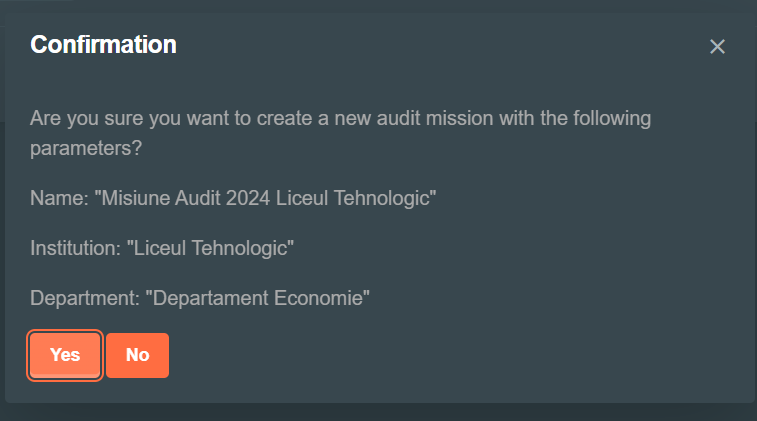
\includegraphics[width=0.5\textwidth]{c1/confirmare_misiune_creata.png}
	\caption{Confirmare creare misiune de audit}
	
\end{figure}


Dupa crearea noii misiuni, auditorul este redirectionat catre o pagina in care acesta poate vizualiza intr-un tabel toate misiunile de audit la care acesta are acces, cele create de el, dar si cele la care i-a fost oferit accesul.Afisarea intrarilor din tabel este una de tip paginata cu un numar de sapte misiuni pe pagina, astfel incat atentia utilizatorului sa fie concentrata doar pe aceste misiuni, in acest fel eliminand posibilitatea de a nu gasi informatia pe care acesa o cauta datorita unui numar prea mare de linii si informatii.
	\vspace{0.5 cm}
\begin{figure}[h]
	\centering
	
	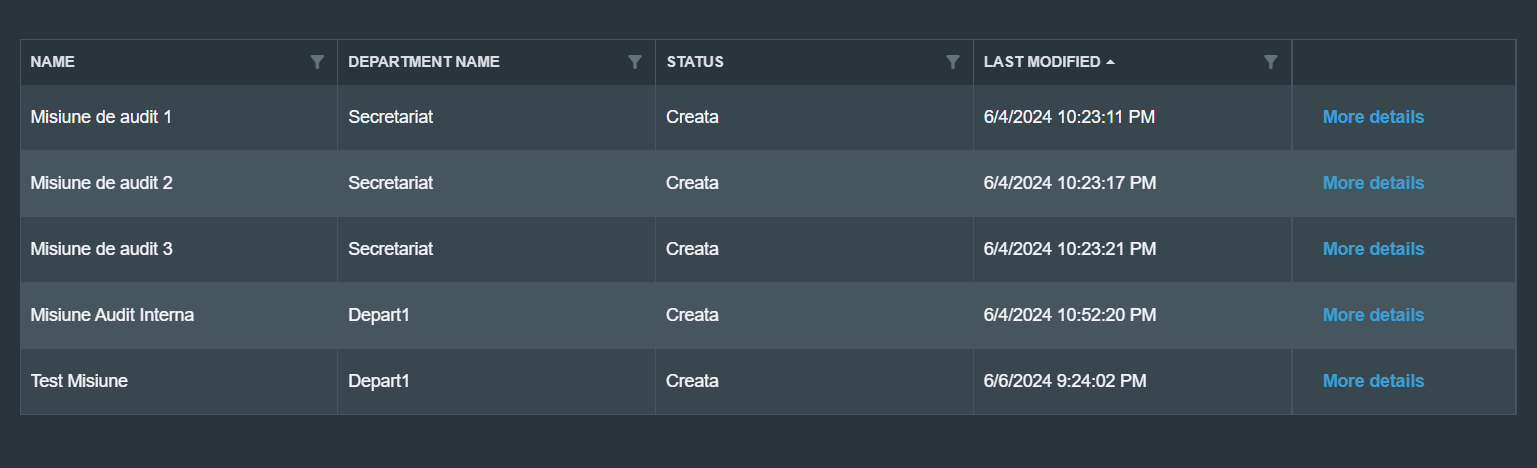
\includegraphics[width=0.8\textwidth]{c1/audit_missions_list.png}
	\caption{Vizualizarea misiunilor de audit}
\end{figure}
De asemenea, informatiile afisate in acest tabel pot fi sortate alfabetic dupa numele misiunii de audit, dupa starea in care fiecare dintre acestea se afla, dupa departamentul asupra caruia se desfasoara misiunea  sau dupa data ultimei modificari a acesteia.

\subsection{Pagina rezumat misiune de audit}

Pagina de rezumat a unei misiuni de audit are ca scop informarea auditorului asupra unei viziuni de ansamblu asupra misiunii de audit respective. Aceasta contine urmatoarele informatii:\\
\begin{itemize}
	
	\item in partea de sus a paginii, auditorului ii este prezentat sub forma unui lant de pasi, statusul curent al misiunii, acesta fiind primul lucru pe care privirea utilizatorului il vede;
		
		\begin{figure}[h]
		\centering
		
		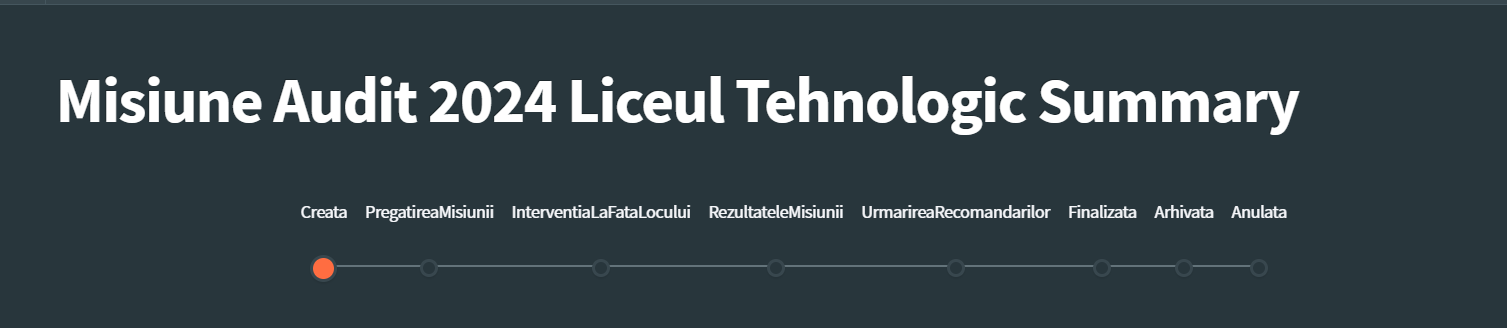
\includegraphics[width=0.9\textwidth]{c1/lant_summary.png}
		\caption{Informatii sumare despre misiunea de audit}
	\end{figure}
	\item o scurta descriere asupra parametrilor misiunii de audit,cum ar fi nume, data ultimii modificari, numele departamentului dar si statusul actual al misiunii. Utilizatorul are optiune de a edita acesti parametri si a salva modificarile aduse;
	
		\vspace{0.5 cm}
	\begin{figure}[h]
		\centering
		
		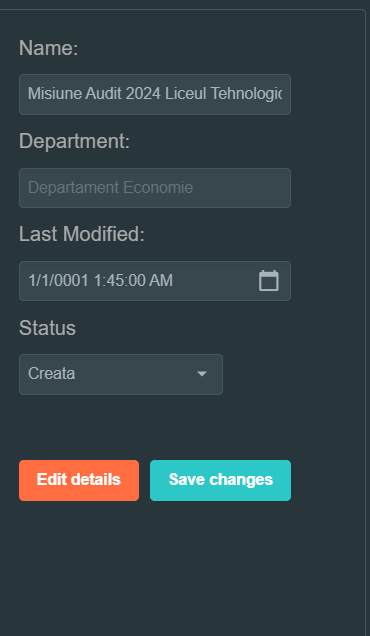
\includegraphics[width=0.5\textwidth]{c1/status_misiune}
		\caption{Informatii sumare despre misiunea de audit}
	\end{figure}
	
	\item in partea dreapta a paginii sunt prezente patru chenare care prezinta cele mai recente modificari si actualizari in materie de : obiective, documente atasate misiunii, fise de identificare a problemei cat si activitati recente asociate misiunii de audit. Utilizatorul are posibilitatea de a naviga apasand pe numele intrarii din lista catre pagina dedicata acesteia, sau la apasarea butonului de 'See more' sa fie redirectionat catre pagina dedicata tututor entitatilor de acel fel;
	\begin{figure}[h]
		\centering
		
		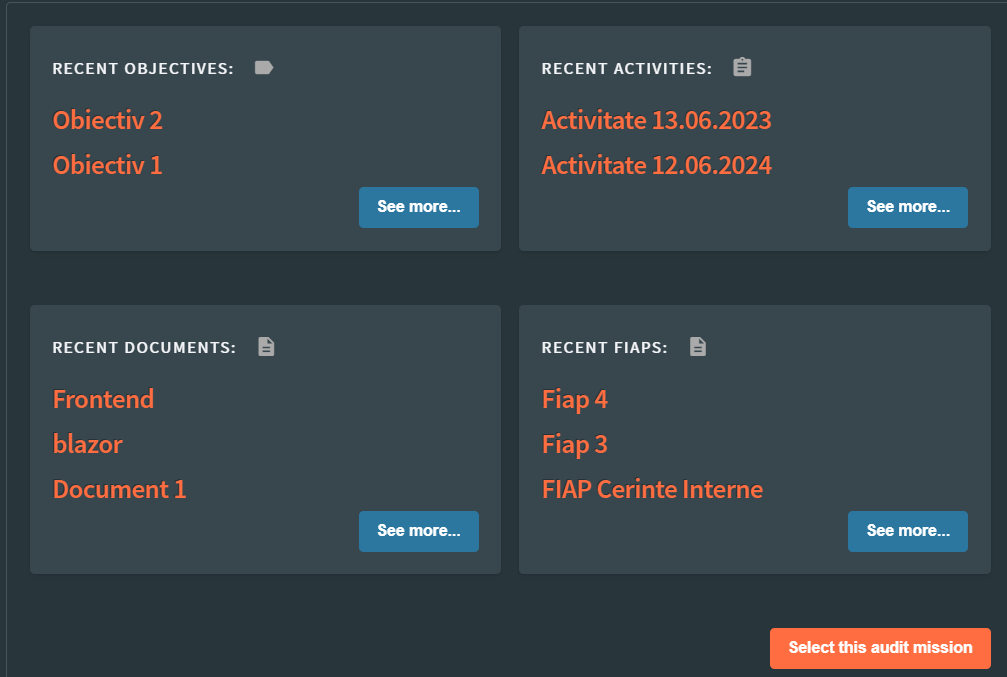
\includegraphics[width=0.7\textwidth]{c1/chenar_recent}
		\caption{Informatii sumare despre modificarile recente}
	\end{figure}
	\item in partea dreapta jos, auditorul are posibilitatea de a selecta misiunea de audit ca fiind misiunea curenta, astfel orice actiune pe care acesta o sa o faca pe platforma o sa ia ca optiune preselectata misiunea selectata de acesta.\\
		
	
\end{itemize}


\subsection{Prelucarea pasilor unei misiuni de audit}

Pentru o reproducere cat mai precisa si cooerenta a stagiilor prin care o misiune de audit trece, platforma permite setarea unui status al fiecarei misiuni de audit, astfel auditorul avand posibilitatea de a-si marca in detaliu progresul pana la momentul curent asupra misiunii de audit.De asemenea, fiecare pas major dintr-o misiune de audit prezinta functionalitati specifice, care vor fi explicate sumar in aceasta subsectiune.
\subsection*{Pregatirea misiunii de audit}
Pregatirea misiunii de audit este etapa initiala in care auditorul creeaza misiunea, consulta misiunile anterioare efectuate la acelasi departament, se elaboreaza un plan de audit, se stabilesc obiectivele, actiunile specifice fiecarui obiectiv respectiv riscurile specifice fiecarei actiuni si se intocmesc o serie de documente oficiale, pentru a tine evidenta activitatilor ulterioare pe care auditorul le va realiza in aceasta misiune de audit.

\subsection*{Interventia la fata locului}
Interventia la fata locului este o etapa importanta a procesului de audit public, etapa care implica de cele mai multe ori o deplasare in teren, auditorul efectueaza interviuri, realizeaza esantioane, analizeaza riscurile si obiectivele stabilite la pasul anterior si incearca sa inteleaga intr-un mod cat mai corect si obiectiv activitatile desfasurate de departamentul respectiv. Acest pas consta in esenta in crearea si completarea a multor documente de tip sablon pe care auditorul le va folosi ulterior in pasii ce urmeaza pentru a intocmi un raport final.

\subsection*{Rezultatele Misiunii}
Dupa finalizarea pasului anterior, auditorul acum dispune de intreg instrumentalul pentru a intocmi un raport final.Acesta este intocmit pe baza diferitelor intalniri intre auditor si repezentantul institutiei in care se discuta aspecte legate de constatarile facute in respectiva misiune de audit. Raportul final cuprinde constatarile facute, recomanandari sub forma 
unor Fise de Identificare si Analiza a Problemei respectiv cauze si consecinte ale problemelor.

Acest raport este prezentat partilor particpante la misiune pentru a le informa asupra rezultatelor misiunii de audit si pentru a ajunge la o intelegere asupra termenilor de remediere a problemelor pe care acestia trebuie sa le rezolve.

\subsection*{Urmarirea recomandarilor}
Urmarirea recomandarilor este pasul final dintr-o misine de audit in care sunt monitorizate recomandarile oferite de catre auditor si respectarea termenilor limita de implementare a acestora. Reprezentatii institutiilor trebuie sa ia la cunostinta aceste recomandari si sa gaseasca, ajutati de Fisa de Identificare si Analiza a Problemei corespunzatoare fiecarei recomandari, solutii pentru fiecare chestiune in parte respectand totodata si termenul liminta impus de aceasta.


\subsection{Stabilirea obiectivelor de auditat}

Stabilirea obiectivelor de auditat are loc in faza initiala a pasului pregatirii misiunii de audit, pas in care auditorul stabileste obiectivele principale care vor fi auditate in cele ce urmeaza. Fiecare obiectiv este compus din mai multe actiuni specifice iar acestea contin la randul lor o serie de riscuri identificate. Aceste riscuri identificate de catre auditor sunt ierarhizate pe baza unei formule de calcul care ia in considerare probabilitatea actiunii de a se intampla, impactul pe care aceasta il va avea si riscul final rezultat al inmultirii celor doua.

Platforma web AudIT ofera aceste functionalitati utilizatorului, astfel incat acesta sa respecte in detaliu toti pasii legislativi ai procedurii de audit public. Auditorul poate forma obiective noi si sa le ataseze la misiunea de audit corespunzatoare.\\

\begin{figure}[h]
	\centering
	
	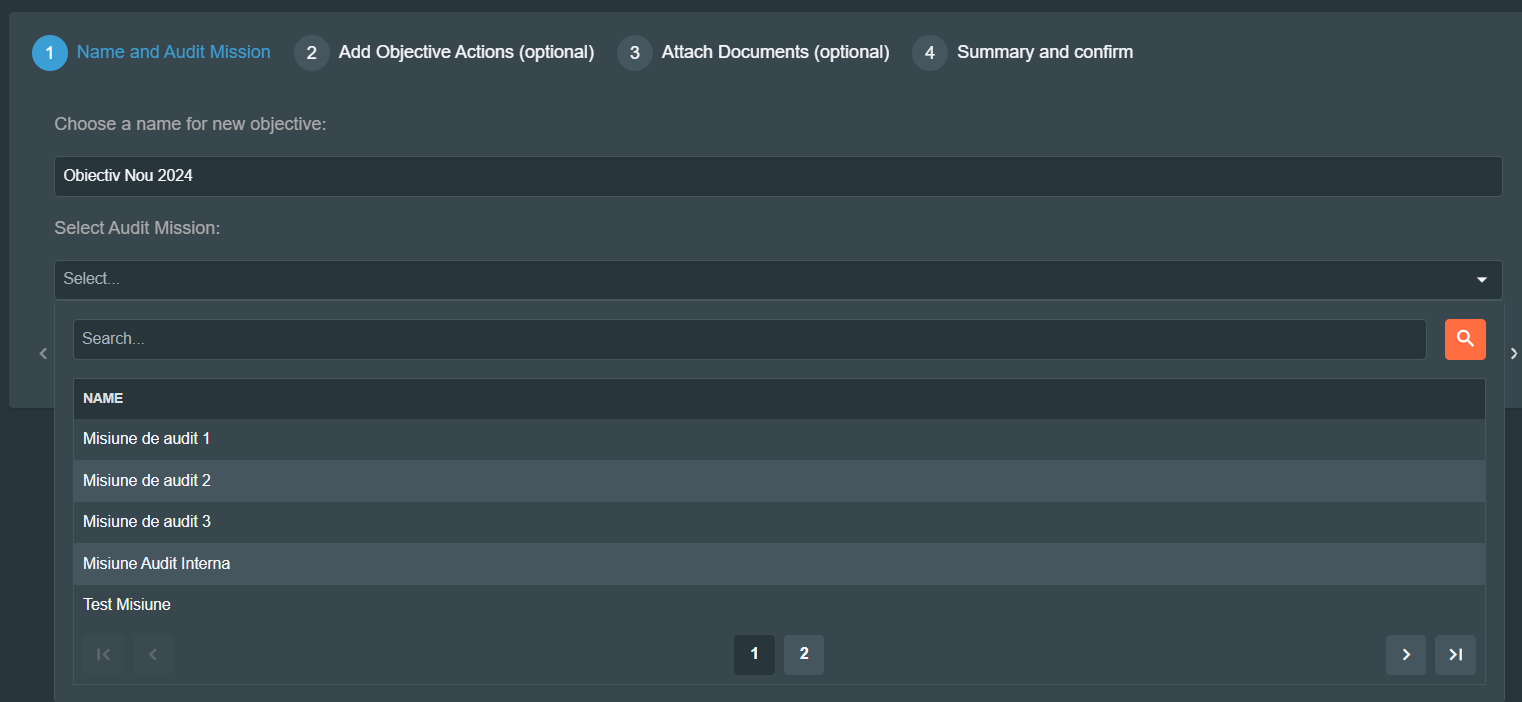
\includegraphics[width=0.8\textwidth]{c1/creare_obiectiv_1}
	\caption{Primul pas in crearea unui nou obiectiv	}
\end{figure}

De asemenea, acesta are posibiliatea de a atasa direct din meniul de creare al unui obiectiv, actiuni specifice obiectibului respectiv, precum si documente necesare sau ajutatore actiunii, astfel usurand semnificativ procesul de inventariere prezent la acest pas.\\
Tot acest proces  de creare a unui nou obiectiv este impartit pe mai multi pasi, astfel incat interactiunea utilizatorului cu aplicatia respectiv cu interfata grafica a acesteia sa fie una cat mai naturala si intuitiva.
\vspace{1cm}
\begin{figure}[h]
	\centering
	
	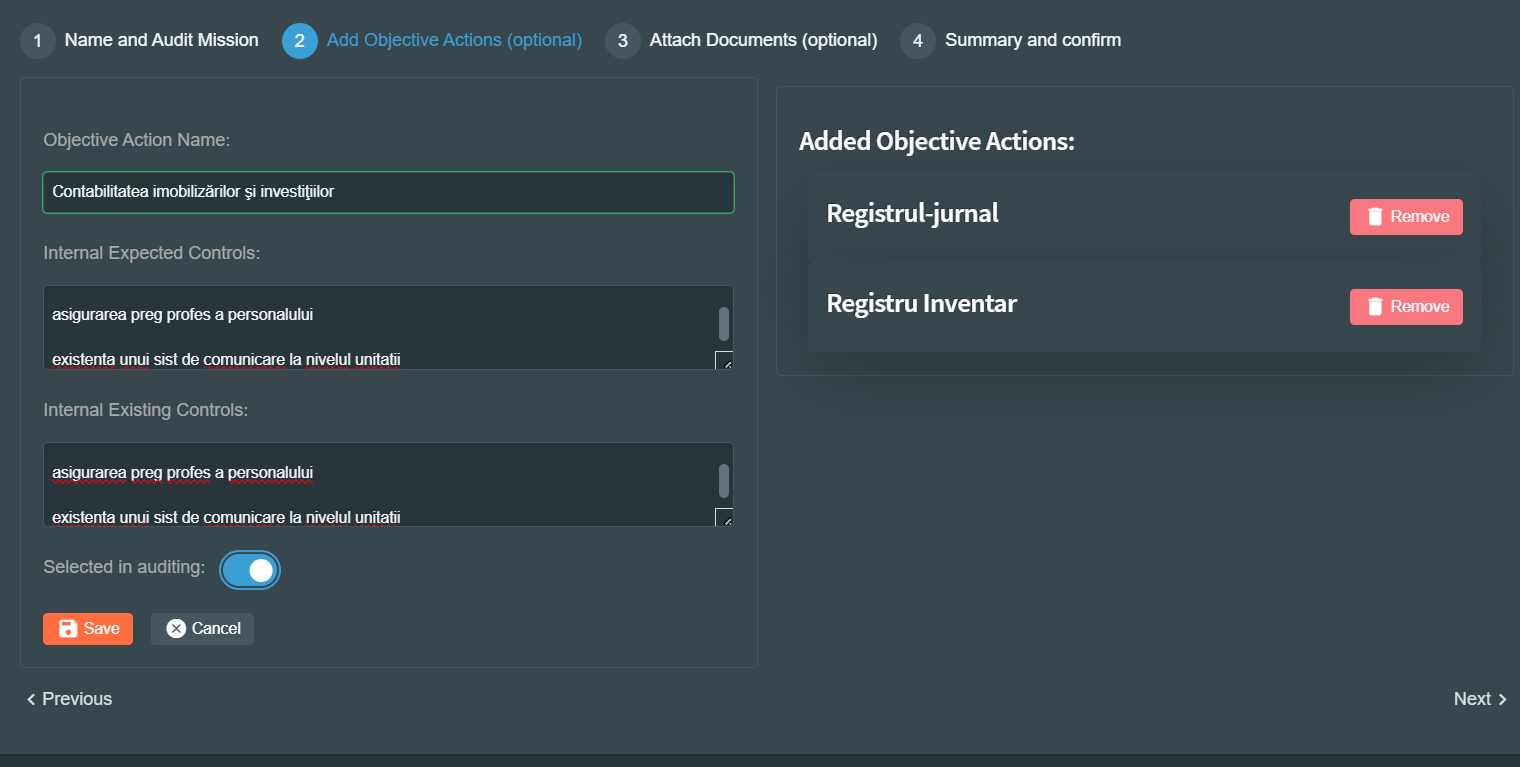
\includegraphics[width=0.9\textwidth]{c1/creare_obiectiv}
	\caption{Atasarea actiunilor specifice unui obiectiv}
\end{figure}

\subsection{Vizualizarea si accesarea ricurilor din misiuni anterioare}
Stabilirea obiectivelor de auditat, fiind un pas relativ important in procesul de audit public, o identificare cat mai precisa si corecta a riscurilor actiunilor acestora este cruciala pentu o buna desfasurare dar si pentru rezultate optime ale misiunii de audit.\\
Aplicatia ofera auditorului acces la un istoric de misiuni de audit public, in care acesta poate filtra doar misiunile de audit asupra departamentului la care se desfasoara si misiunea de audit curenta, astfel avand posibilitatea de analiza a riscurilor ce deja au fost descoperite, ajutandu-l 
astfel pe acesta sa stabileasca noi riscuri relevante, corecte si in conformitate cu situatia actuala.

\subsection{Identificarea si evaluarea riscurilor}
Platforma AudIT pune la dispozitia utilizatorului un mecanism de stabilire a riscurilor, acestia avand posibilitatea de a atasa noi riscuri identificate la o actiune, de a edita valorile riscurilor deja prezente sau de a sterge un risc din tabel in cazul in care acesta nu mai este conform sau o greseala in definirea acestuia a fost depistata.

Aceasta functionalitate este implementata prin intermediul unui tabel paginat, fiecare linie afisand informatii relevante despre risc, cum ar fi probabilitatea, impactul, scorul final (riscul propriu zis) dar si o scurta descriere a acestuia.

\vspace{1cm}
\begin{figure}[h]
	\centering
	
	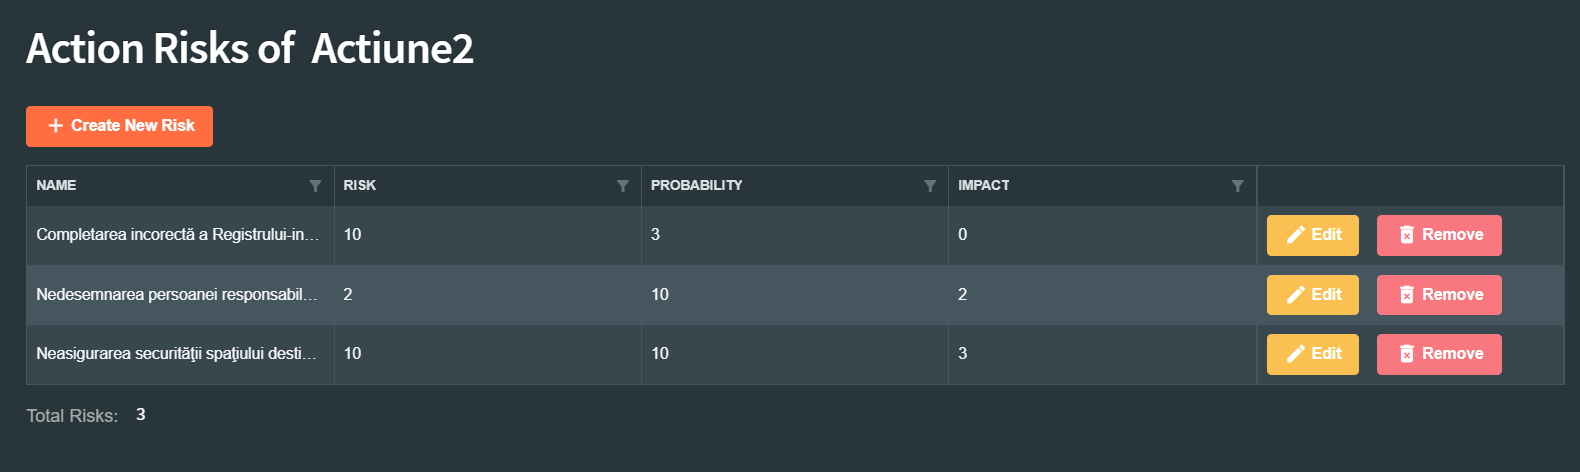
\includegraphics[width=0.9\textwidth]{c1/tabel_riscuri}
	\caption{Informatii sumare despre riscurile}
\end{figure}

De asemenea, in partea de jos a tabelului este afisat si numarul total de riscuri atasate actiunii respective, cat si scorul total al tuturor riscurilor, scor care il va ajuta ulterior pe auditor in stabilirea selectarii sau nu a obiectivul in auditare.

\subsection{Vizualizarea obiectivelor}

Ulterior crearii unui nou obiectiv al misiunii de audit, utilizatorul este redirectionat catre o pagina in care acesta poate viziona prin intermediul unui tabel toate obiectivele deja stabilite pentru misiunea respectiva de audit intr-un format cat mai intuitiv, usor de folosit si inteles .

Auditorul poate vizualiza toate actiunile specifice obiectivului pe care il analizeaza, avand in plus si informatii asupra numelui, data ulitimii modificari/accesari a acesteia, daca este selectat sau nu in procesul de auditare sau optiunea de a inspecta toate riscurile identificate pana la momentul curent, prin apasarea butonului 'More details' din dreptul coloanei 'Action Risks Details'.

\vspace{1cm}
\begin{figure}[h]
	\centering
	
	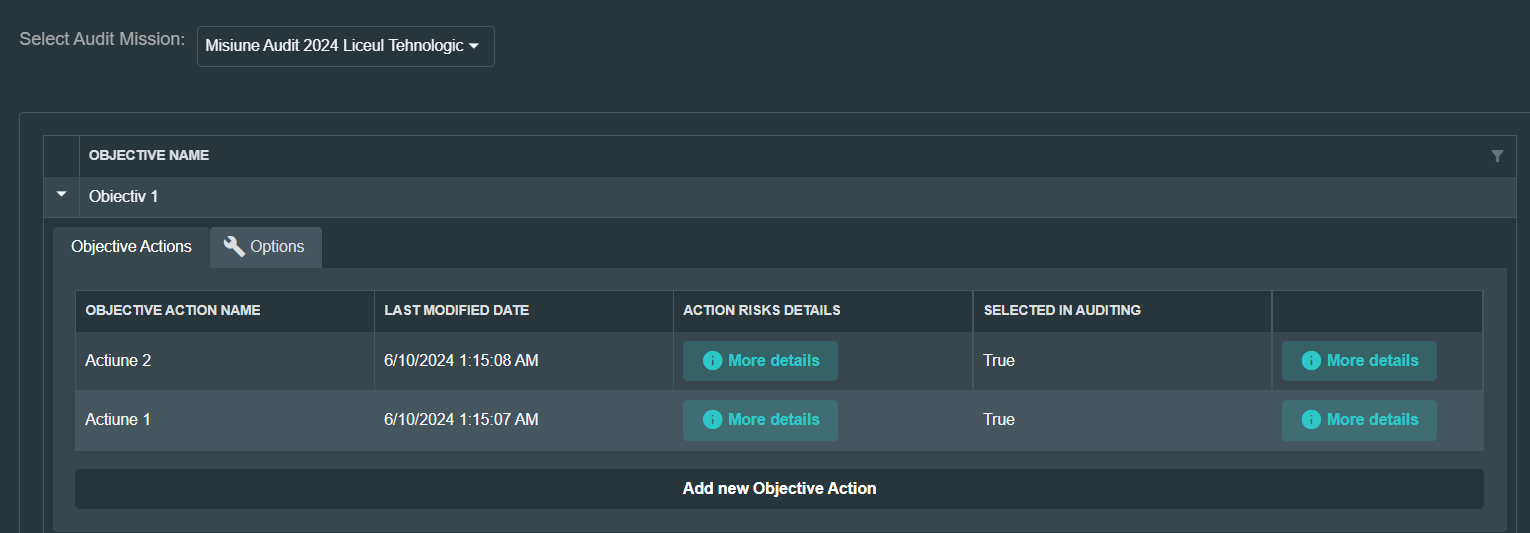
\includegraphics[width=1\textwidth]{c1/tabel_obiective}
	\caption{Informatii despre obiectivele misiunii de audit}
\end{figure}



De asemenea, utilizatorul poate naviga prin apasarea butonului 'More details' din dreptul ultimii coloane catre pagina dedicata detaliilor actiunii, in care acesta poate gasi mai multe amanunte referitoare la actiunea selectata.


\vspace{1cm}
\begin{figure}[h]
	\centering
	
	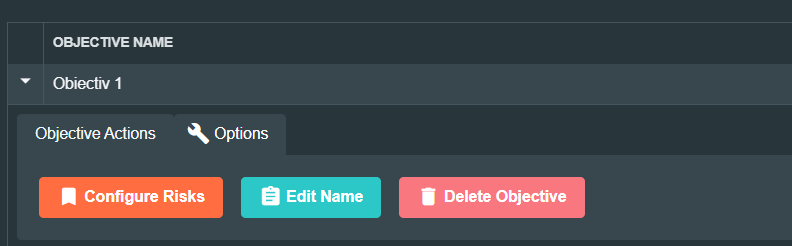
\includegraphics[width=0.9\textwidth]{c1/optiuni_suplimentare}
	\caption{Optiuni suplimentare gestionare obiectiv}
\end{figure}


\subsection{Pagina detalii actiune}
Pagina ofera auditorului o imagine de ansamblu asupra actiunii selectate, astfel acesta poate accesa si vizualiza detalii despre actiune cum ar fi:\\
\begin{itemize}
	\item un scurt rezumat al acesteia care contine numele, daca este sau nu selectata in procesul de audit, o lista de Controale Interne Asteptate respectiv o lista de Controale Interne Existente;
	
	\item  un tabel in care sunt afisate intr-un mod paginat riscurile asociate cu actiunea respectiva, afisand informatii despre impact,probabilitate si scorul riscului;
	
	\item  un tabel care contine informatii despre diferite FIAP-uri (Fisa de Identificare si Analiza a Problemei) care sunt asociate cu actiunea, afisand informatii despre numele FIAP-ului, perioada de start si de sfarsit a interactiunii, problema, cauza si recomandarea oferita de auditor;
	
	\item  un tabel  in care sunt afisate activitatile desfasurate de auditor avand ca motiv actiunea detaliata pe pagina, tabelul prezentand informatii despre numele activitatii, numele departamenutului asupra caruia a avut loc dar si tipul actiunii;
	
\end{itemize}


\vspace{1cm}
\begin{figure}[h]
	\centering
	
	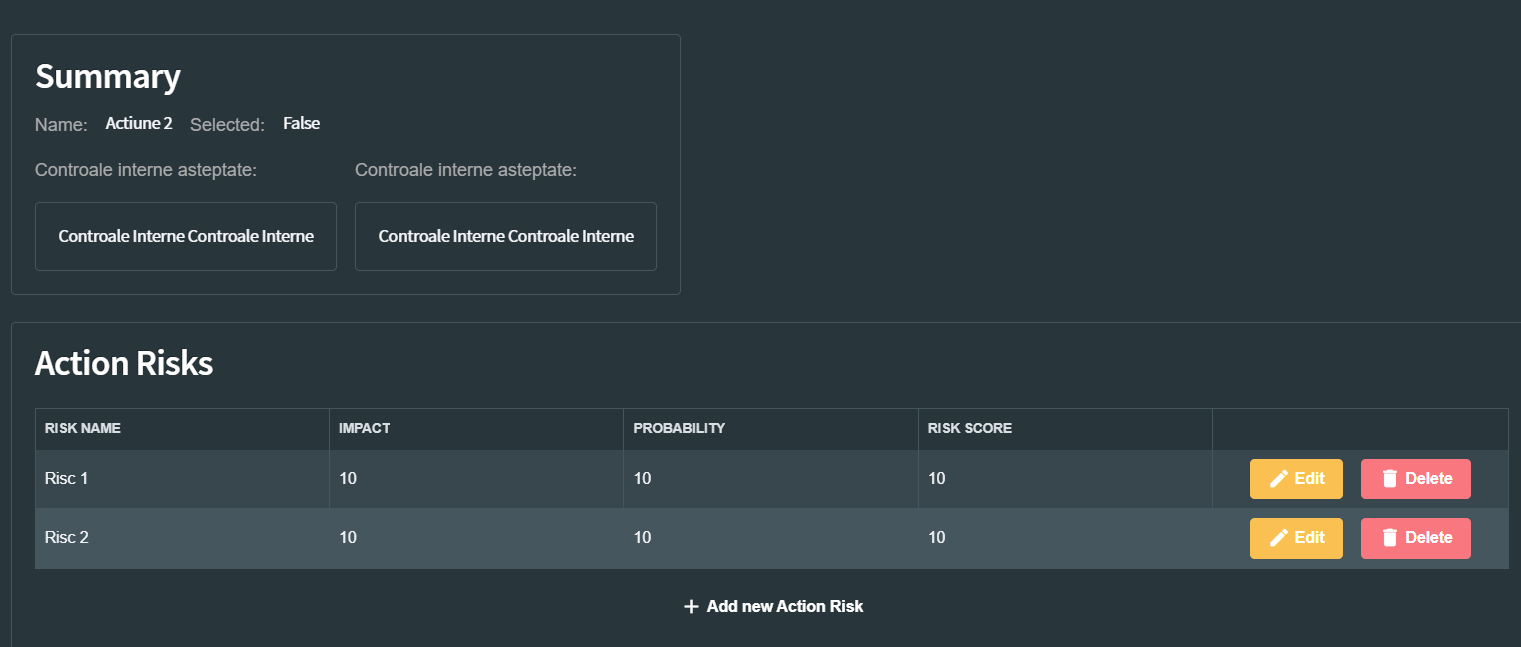
\includegraphics[width=0.9\textwidth]{c1/obiectiv_summary}
	\caption{Informatii despre obiectivul selectat}
\end{figure}


De asemenea, in partea de jos a fiecarui tabel, utilzatorul are optiunea de a adauga o noua entitate prin apasarea butonului 'Add new'.La apasarea acestuia, se deschide un dialog de tip 
form in care utilizatorul poate completa campurile pentru a initializa o noua intrare in tabel.

\vspace{1cm}
\begin{figure}[h]
	\centering
	
	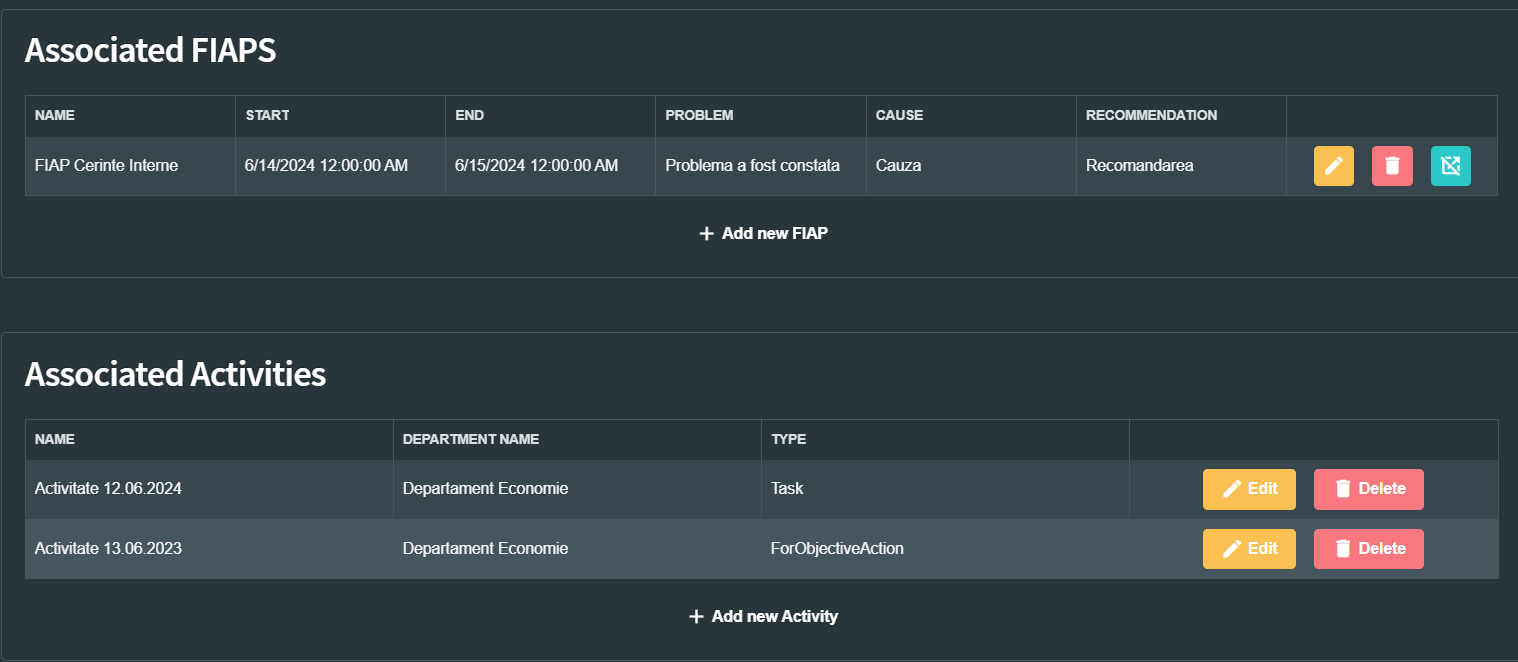
\includegraphics[width=0.9\textwidth]{c1/obiectiv_summary2.png}
	\caption{Informatii FIAP si Activitati}
\end{figure}


\subsection{Salvarea documentelor necesare pe platforma}

Inventarierea si accesarea documentelor necesare pentru desfasurarea unei misiuni de audit public este o etapa esentiala pentru asigurarea transparentei si eficientei procesului de audit public.

Platforma AudIT ofera aceste functionalitati utilizatorilor acesteia, astfel incat atat un auditor cat si membri ai departamentelor auditate care au acces la misiunea de audit, sa poata incarca si salveze pe platforma orice tip de document ce nu depaseste o anumita marime in dimensiune prestabilita.

La incarcarea unui astfel de document, auditorul are posibilitatea de a alege intre tipul documentului incarcat: document standard(un fisier de sine statator deja completat) sau document sablon(un fisier care necesita completarea acestuia inainte sau ulterior salvarii acestuia pe platforma).\\

---INSERT PIC HERE --- \\




 \subsection{Accesarea documentelor necesare pe platforma}
 
 Dupa crearea unui document si salvarea acestuia pe platforma, utilizatorii au optiunea de a vizualiza documentele elaborate de acestia respectiv cele la care li s-a oferit accesul.
 
 Afisarea documentelor se face prin intermediul unui tabel, unde sunt afisate informatii cum ar fi: numele documentului, tipul documentului, misiunea de audit de care apartine, starea in care acesta se afla, ultima data la care acesta a fost modificat si numele departamentului caruia ii este adresat (in cazul documentelor sablon).
 
 De asemenea, intrarile din tabel pot fi filtrate si sortate dupa diferite criterii, spre exemplu : alfabetic dupa numele sau tipul documentului, dupa starea in care acesta se afla sau dupa numele misiunii de audit de care acesta apartine.\\
 
 ---INSERT PIC HERE---\\
 
 
 \subsection{Completarea documentelor tip sablon}
 
	Una dintre sarcinile de baza ale auditorului, dar si un punct nevralgic al sistemului de audit public despre care am discutat anterior, il constituie nevoie de a inventaria si de a completa numeroase documente de tip sablon. Avand in vedere faptul ca numarul acestor documente este uneori de ordinul zecilor intr-o misiune de audit, o functionalitate care ar permite auditorului sa completeze in mediul digital acest tip de documente ar fi bine venita.
	
	Platforma AudIT ofera posibilitatea utilizatorilor sa completeze si sa editeze direct in aplicatie documentele de tip sablon salvate de acestia. Functionalitatea este implementata prin utilizarea unui simplu 
	MarkDown editor, in care documentul sablon este incarcat, editat, iar la finalizarea procesului, schimbarile facute sunt salvate.\\
	
	--INSERT PIC HERE ---\\
	
	\subsection{Bara de navigare}
	Pentru facilitarea unui acces cat mai usor la principalele functionalitati ale platformei, utilizatorul se poate folosi de bara de navigare prezenta intotdeauna in partea stanga a aplicatiei.
	
	Aceasta este impartita in sectiuni specifice fiecarei entitati, astfel incat mentionam:
	\begin{itemize}
		\item  sectiunea misiunilor de audit unde regasim optiunea de a crea o noua misiune de audit, de a naviga la misiunea de audit selectata curent, vizualiza lista de misiuni de audit dar si o optiune de a cauta in fuctie de numele misiunii de audit; 
		
		\item sectiunea obiectivelor in care exista optiunile de creare a unui nou obiectiv, navigare catre pagina tututor obiectivelor, crearea a noi actiuni specifice unui obiectiv dar si posibilitatea de a cauta un obiectiv al misiunii de audit curente in functie de numele acestuia;
		
		\item sectiunea recomandarilor unde auditorul poate adauga o noua recomandare dar si vizualiza recomandarile deja existente;
		
		\item sectiunea documentelor unde similar, merg adaugate noi documente si vizualiza documente deja existente pe platforma;
		
		\item sectiunea activitatilor unde utilizatorul poate consemna activitati noi desfasurate sau naviga spre cele existente deja;
		
		\item sectiunea dedicata exportarii, unde auditorul poate naviga spre diferite pagini de convertire a obiectivelor, actiunilor si a riscurilor in diferite formate dar si autocompletare a unor documente oficiale de tip sablon, cum ar fi Fise de Identificare a Problemei sau Raport de Evaluarea a Riscurilor;
		
		\item sectiunea de control al accesului, unde auditorul sau reprezentantii institutiilor audidate pot consulta resursele la care au acces de scriere sau citire respectiv a oferi acces altor utilizatori la resurse personale;
		
		\item sectiunea de configurare, unde un utilizator cu drepturi elevate poate configura institutiile respectiv departamentele inregistrate pe platforma, adaugand, editand sau eliminand instante dintre acestea.
		
		
		
		

	\end{itemize}
\newpage
   De asemenea, bara de navigare se actualizeaza in functie de statusul de autentificare si rolul pe care utilizatorul il are.
   \begin{figure}[h]
   	\centering
   	\begin{minipage}{.5\textwidth}
   		\centering
   		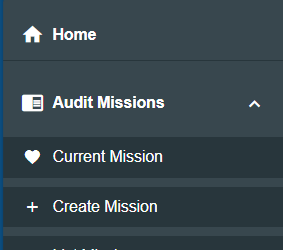
\includegraphics[width=.9\linewidth]{c1/navbar_logat}
   		\caption{Utilizator autentificat}
   		
   	\end{minipage}%
   	\begin{minipage}{.5\textwidth}
   		\centering
   		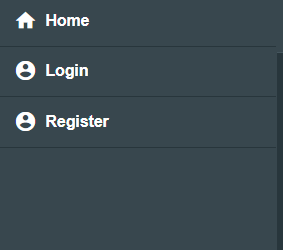
\includegraphics[width=.9\linewidth]{c1/navbar_nelogat.png}
   		\caption{Utilizator neautentificat}
   		
   	\end{minipage}
   	
   	
   \end{figure}

	\subsection{Gestionarea accesului la resurse partajate}
	
	 O componenta cheie in desfasurarea corecta a unei misiuni de audit este colaborarea intre partile participante la misiunea de audit.
	 
		Functionalitatea de acordare a accesului la resurse, contribuie la o colaborare cat mai stransa intre membrii partipanti la misiunea de audit, astfel un auditor poate acorda acces de scriere sau citire la diferite resurse create de acesta.
		
		In plus, o lista completa a accesului primit sau oferit se poate vizualiza de catre utilizator pe o pagina dedicata, unde sub forma unui tabel sunt prezentate informatii specifice cum ar fi numele si tipul resursei si email-ul utilizatorului caruia i s-a oferit  acces
		
	\subsection{Gestionarea activitatilor desfasurate}
	 Prin aceasta functionalitate, auditorul poate consemna orice sarcina pe care acesta o efectueaza pe platforma prin intermediul unei activitati. Aceasta cuprinde informatii referitoare la actiunea asupra careia s-a efectuat o activitate, departamentul asociat dar si tipul activitatii care poate fi asociat unei misiuni, unei actiuni sau pur si simplu o sarcina administrativa.
	 
	 De asemenea , toate activitatile consemnate intr-o misiune de audit, pot fi vizualizate de catre auditor intr-o pagina dedicata, acestea fiind afisate prin intermediul unui tabel care ofera informatii referitoare la numele acesteia, tipul actiunii sau departamentul asupra cauia s-a realizat respectiva sarcina.
	 
	
	\subsection{Profilul personal}
	Pagina profilul personal este locul unde utilizatorul poate sa isi verifice informatiile personale care sunt disponibile pe platforma avand posibilitatea de a le edita. Informatiile cuprind detalii de contact, cum ar fi adresa de email, numar de telefon al institutiei, numar de telefon personal, adresa fizica de contact respectiv daca acesta este verificat sau nu.
 
	
	\subsection{Sistemul de notificari}
		Functionalitatea permite vizualirea notificarilor in ceea ce priveste crearea de noi resurse, primirea accesului la o anumite resursa sau notificari in ceea ce priveste actualizarea sau implementarea unor solutii la recomandarile impuse de auditor din partea reprezentantilor institutiei asupra careia are loc misiunea de audit.


	\section{Solutii similare}
	Solutia descrisa nu este o idee unica, dar este esential sa studiem si sa intelegem modul in care solutiile similare abordat aceasta problema, avand astfel posibiliatea sa identificam puncte forte cat si puncte slabe ale aplicatiei ce merg ulterior imbunatatite, inovand acolo unde este posibil.
	
	In sectiunea urmatoare o sa fie prezentate cateva solutii similare adresate problemei de digitalizare in domeniul auditului public si o sa fie analizate functionalitatile forte ale acestora. 
	
	\subsection*{Audit Pro}
	
	Audit Pro este o aplicatie dezvoltata in special pentru sistemul de operare Windows si care incearca sa ofere un mediu de lucru doar auditorilor din institutiile publice.\\
	Solutia oferita este una care se bazeaza pe achizitionarea acesteia contra unui pret, oferid in pachet si o configurare initiala a institutiilor si membrilor din departamentul de audit.
	
	Aceasta ofera functionalitati similare cu solutia descrisa in acest document, dar printre care se evidentiaza: 
	\begin{itemize}
		\item accesul la un calendar unde auditorul poate vizualiza evenimentele importante ce vor avea sau au avut loc, avand de asemenea posibilitatea de a adauga noi evenimente in acesta;
		
		\item o pagina dedicata analizei costurilor desfasurarii anumitor activitati specifice unei misiuni de audit: costuri de deplasare, diurne etc;
		
		\item un meniu de ajutor unde utilizatorul poate accesa informatii ajutatoare in vederea utilizarii anumitor functionalitati din aplicatie;
		
	\end{itemize}
	
	\vspace{1cm}
	\begin{figure}[h]
		\centering
		
		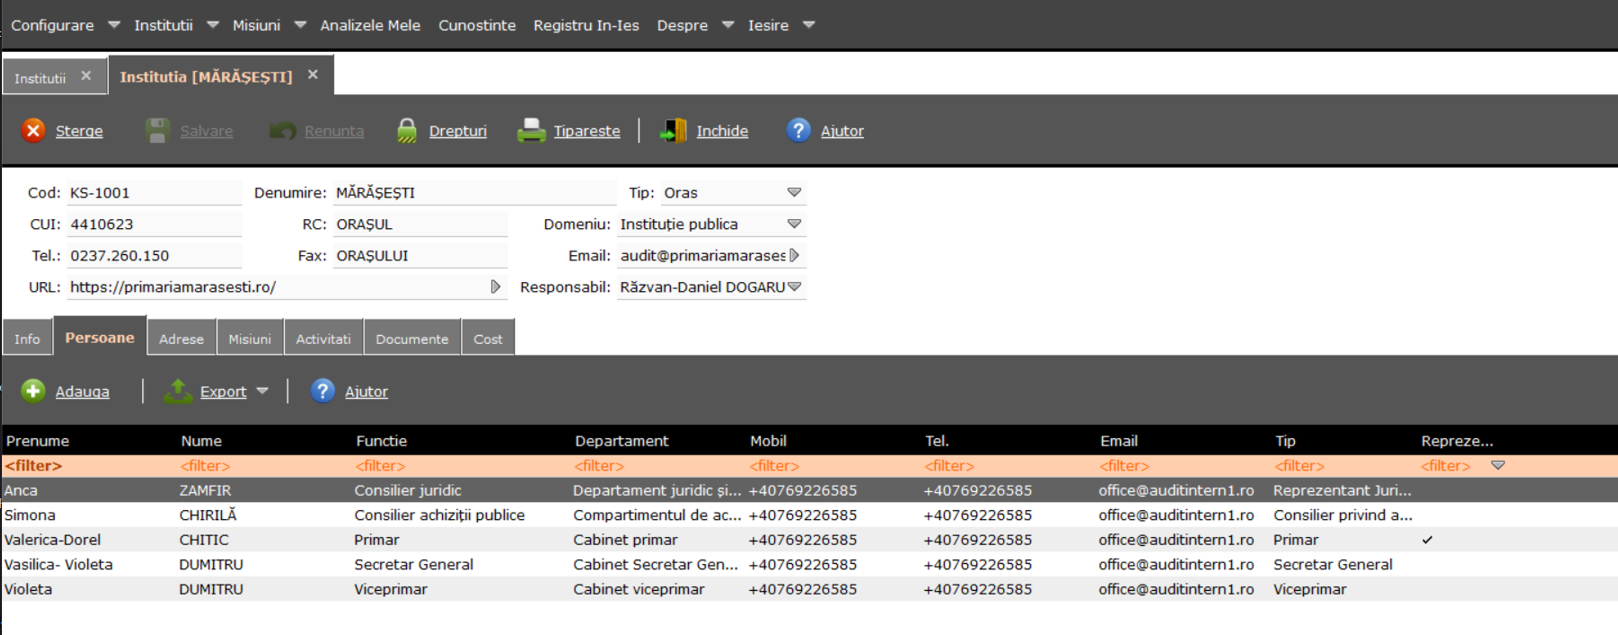
\includegraphics[width=0.9\textwidth]{c1/auditpro1}
		\caption{Tabel din aplicatia Audit Pro}
	\end{figure}
	
	
	
Pe de alta parte, solutia descrisa prezinta si anumite dezavantaje care constau in modul in care aceasta a fost implementata, unul dintre acestea fiind limitarea strict la utilizarea acesteia numai pe sistemul de operare Windows, marginind in acest mod alte sisteme de operare prezente.
De asemenea, din punctul meu de vedere, aspectul grafic si interfata pe care aceasta solutie o prezinta nu este una foarte intuitiva si poate induce in eroare utilizatorii in anumite situatii.
\vspace{1cm}
\begin{figure}[h]
	\centering
	
	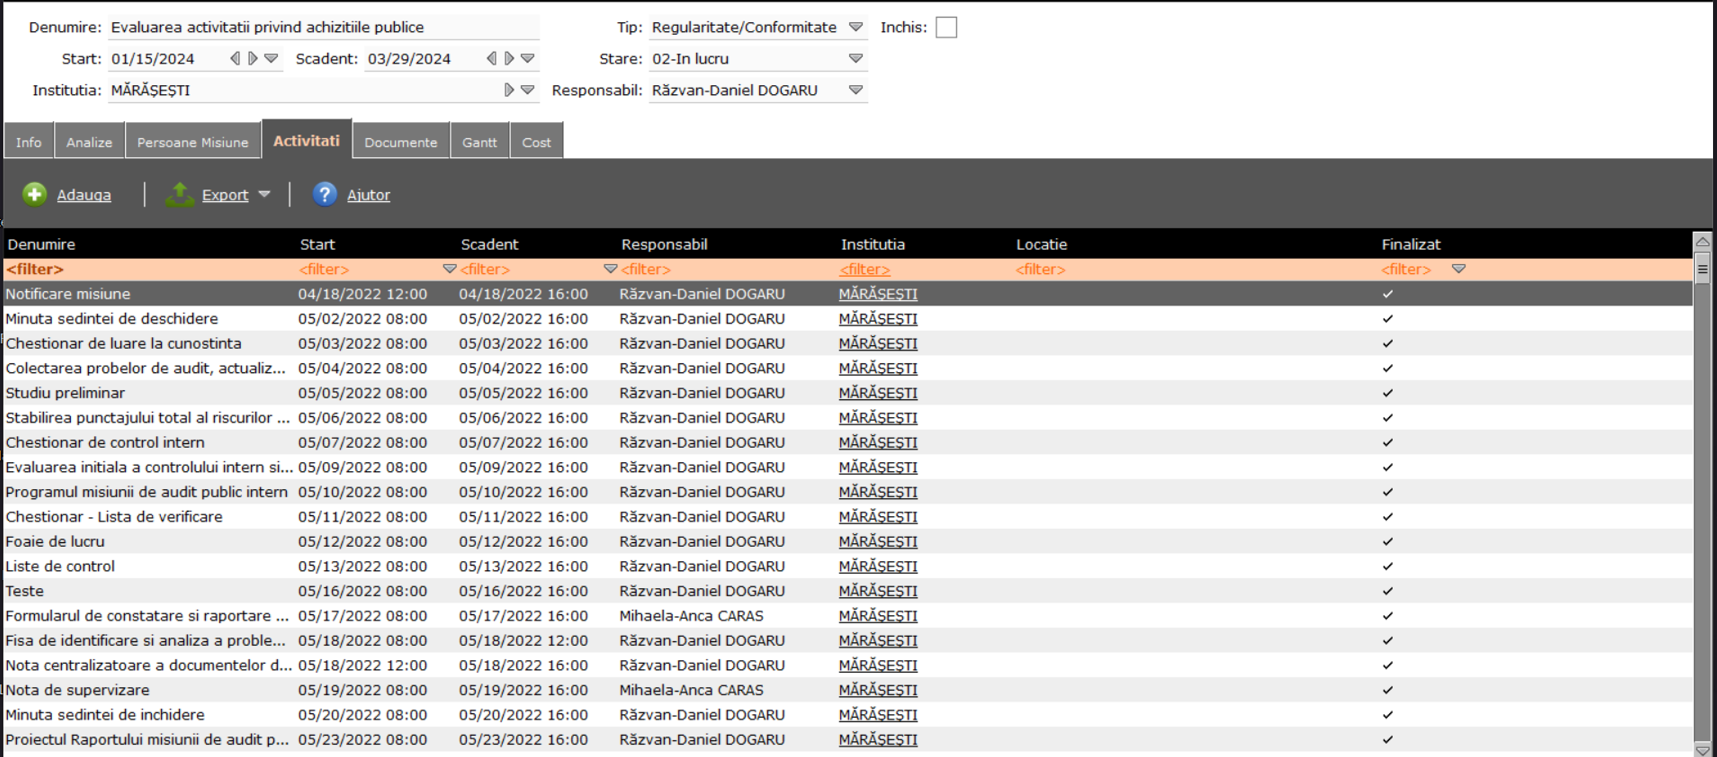
\includegraphics[width=0.9\textwidth]{c1/auditpro2}
	\caption{Tabel din aplicatia Audit Pro}
\end{figure}

	\newpage
	\subsection*{Site Audit Pro }
	
	Chiar daca numele este similar cu solutia prezentat similar, este vorba despre un alt proiect, de aceasta data o platforma web cu suport si pentru aplicatie mobila care prezinta solutii pentru auditul in sectorul privat, cel al companiilor.
	Din informatiile prezente pe pagina  lor de prezentare, se poate trage concluzia ca aceasta solutie este una ajunsa la maturitate, primind constant actualizari in ceea ce priveste functionalitatile oferite de aceasta.
	 
	Dintre numeroasele facilitati pe care aceasta solutie le ofera, cele mai importante si cu un impact mai mare ar putea fi:
	\begin{itemize}
		\item posibilitatea de a lucra in mediul \textit{offline} pe platforma mobila, informatiile fiind actualizate cu server-ul principal in momentul in care exista o conexiune la internet;
		
		\item sincronizarea proiectelor pe toate dispozitivele (Web, Android si IOS) astfel incat toate informatiile sa fie actualiate in timp real;
		
		\item organizarea proiectelor si resurselor in directoare, facilitand astfel o navigare mai eficienta ;
	\end{itemize}
	\begin{figure}[h]
		\centering
		
		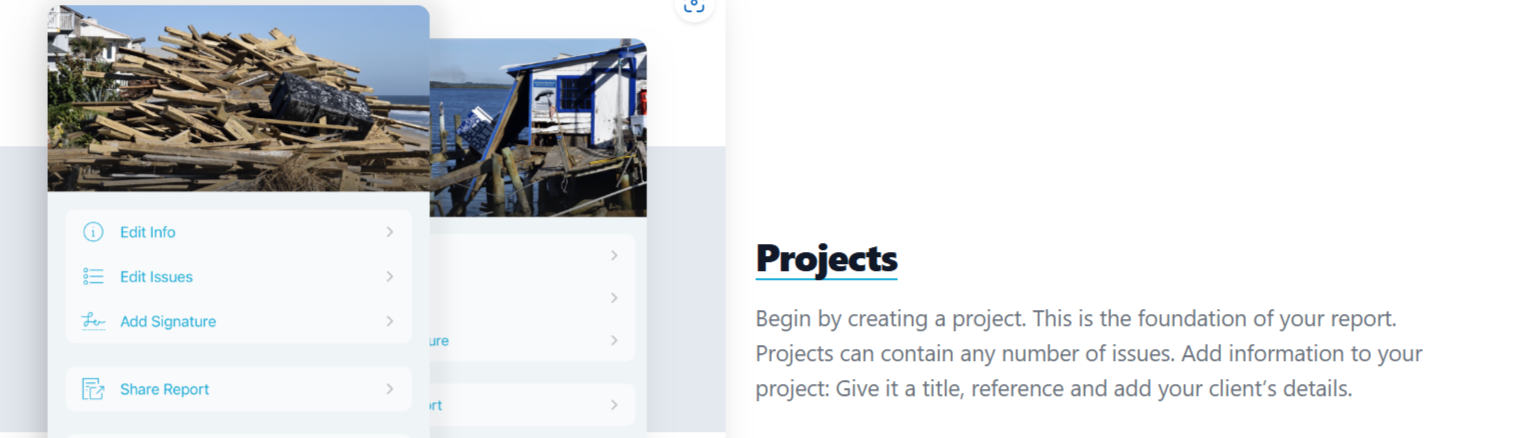
\includegraphics[width=0.6\textwidth]{c1/auditpro3}
		\caption{Tabel din platforma Site Audit Pro}
	\end{figure}
	
	Cu toate acestea, un dezavantaj pe care aceasta solutie il ofera este acela ca procedurile pe care acesta este construit, nu se muleaza si nu corespund in cea mai mare parte cu cele din sistemul de audit public din Romania, utilizatorii trebuind astfel sa se adapteze si sa incerce pe cat posibil sa personalizeze si sa modifice functionalitatile oferite de acestia.
	
	
	
	
